\documentclass[12pt]{article}
\usepackage[a4paper,margin=1in]{geometry}
\usepackage[T1]{fontenc}
\usepackage[utf8]{inputenc}
\usepackage{graphicx}
\usepackage{booktabs}
\usepackage{enumitem}
\usepackage{setspace}
\usepackage{float}
\usepackage{xcolor}
\usepackage{amsmath}

\title{\textbf{Mirror Reflection Agent: A Structured Reliability-Control Architecture with Pilot Evidence for Scientific Reasoning}}
\author{Brook \\ Independent Researcher}
\date{}

\begin{document}
\maketitle
\onehalfspacing
\emergencystretch=2em

\begin{abstract}
Large language models are increasingly used in scientific workflows, yet their practical value remains constrained by unsupported certainty, weak handling of conditional evidence, and poor retention of prior corrections. We present Mirror Reflection Agent, a reliability-oriented architecture that separates candidate cognition from final output and inserts an explicit mirror-critique stage between them. The system constructs a structured intermediate state, critiques it with typed verdicts such as revise, retrieve, wait, diverge, and pass, and stores correction lineage and reusable strategy signals in memory. Unlike prompt-only self-refinement pipelines, the proposed architecture externalizes intermediate cognition and makes revision control auditable. We instantiate the design with scientific and commonsense knowledge layers, a deterministic critique module, project-local memory, optional dual-layer memory, and replayable run audits. The contribution is not a claim about machine consciousness or subjective awareness, but a practical control mechanism for safer reasoning. We report pilot evidence from the current repository benchmark, where the dual-layer setting reduces premature convergence and improves correction retention relative to a local-only setting. The paper therefore makes a bounded claim: the present implementation demonstrates a proof-of-mechanism for reliability control, while a larger science-facing benchmark remains future work.
\end{abstract}

\noindent\textbf{Keywords:} scientific reasoning, reflective agents, reliability control, memory, uncertainty, metacognition

\section{Introduction}

Scientific use of large language models requires more than fluent answers. A useful system must distinguish strong evidence from weak prior knowledge, preserve source conditions, reduce unsupported certainty, and remember prior corrections without blindly repeating them. Existing agent pipelines often improve outputs by adding reflection or retrieval, but they still leave three recurring problems:

\begin{itemize}[leftmargin=1.2em]
\item intermediate reasoning is not represented as an inspectable object
\item critique outcomes are not encoded as explicit control decisions
\item prior corrections are not preserved as structured reusable lineage
\end{itemize}

This paper addresses those gaps with Mirror Reflection Agent, a structured reliability-control architecture. Rather than directly producing a final answer, the system builds a candidate cognitive state, critiques it with a mirror layer, and then either revises, retrieves memory, diverges to a new scaffold, defers, or finalizes. The design is engineering-oriented and auditable. It does not claim subjective awareness, consciousness, or human-like introspection. Its core claim is narrower and testable: explicit cognitive state plus typed critique plus correction-lineage memory can improve reliability-oriented behavior in scientific and science-adjacent reasoning tasks. The current manuscript supports that claim at the level of pilot mechanism evidence rather than broad task-general performance.

\section{Related Work and Positioning}

Mirror Reflection Agent sits at the intersection of self-refinement, reflective agents, retrieval-augmented generation, and reliability-oriented AI for Science systems. Prior work such as Self-Refine and Reflexion showed that iterative self-feedback can improve outputs, while CRITIC and Self-RAG demonstrated the value of critique and retrieval in controlled generation. The present work differs in emphasis. It does not primarily contribute a new prompting trick or a new retrieval policy. Instead, it contributes an explicit reliability-control structure in which intermediate cognition is externalized, critique outcomes are typed, and correction lineage is preserved as reusable memory.

The architecture should also be distinguished from generative adversarial networks. GANs optimize a generator against a discriminator during training, usually to improve distributional realism. Mirror Reflection Agent does not implement adversarial training and does not learn by generator-discriminator competition. Its mirror layer is a run-time oversight module that evaluates a structured candidate state and emits a control decision for revision, retrieval, abstention, or finalization. The relevant contrast is therefore not adversarial learning versus self-reflection, but training-time realism optimization versus inference-time reliability governance.

The architecture also invites comparison to historical introspective traditions, including Buddhist Yogacara or consciousness-only thought, because both are concerned with how internal representations mediate what appears as knowledge. In this paper, that comparison is used only as a conceptual analogy. It does not serve as engineering evidence, proof of subjective awareness, or validation of philosophical claims. The system is a practical control architecture, not a theory of mind.

\begin{table}[H]
\centering
\begin{tabular}{p{3.0cm}p{2.1cm}p{2.2cm}p{2.5cm}p{2.2cm}}
\toprule
Method & Externalized state & Typed control verdicts & Persistent correction lineage & Abstention governance \\
\midrule
Self-Refine & limited & no & no & no \\
Reflexion & partial verbal memory & no & partial episodic memory & limited \\
CRITIC & tool-grounded critique & no & no & limited \\
Self-RAG & retrieval-aware generation & partial retrieval token control & no & limited \\
Mirror Reflection Agent & explicit \texttt{MindState} & yes & yes & yes \\
\bottomrule
\end{tabular}
\caption{Positioning of the present work against closely related reflective pipelines. The table isolates the paper's intended novelty as the combination of explicit state externalization, verdict typing, correction-lineage memory, and abstention-oriented control.}
\label{tab:related-work}
\end{table}

\section{Core Contribution}

The deepest contribution of the architecture is not generic self-reflection. It is the conversion of reliability problems into explicit state and explicit control flow. The architecture contributes three linked mechanisms:

\begin{enumerate}[leftmargin=1.4em]
\item \textbf{State externalization.} Candidate reasoning is represented as a structured \texttt{MindState} with claim, evidence, assumptions, alternatives, confidence, and risk.
\item \textbf{Verdict-typed oversight.} Critique is represented as a structured \texttt{MirrorVerdict} with explicit actions: \texttt{pass}, \texttt{revise}, \texttt{retrieve}, \texttt{wait}, and \texttt{diverge}.
\item \textbf{Correction-lineage memory.} Memory stores not only facts, but also prior bias alerts, correction actions, and reusable strategies.
\end{enumerate}

This makes the system materially different from prompt-only reflection. The mirror is not just another text prompt. It is a decision layer that governs whether the system should answer, revise, retrieve, or abstain.

\section{Architecture}

The system follows:

\begin{center}
\texttt{input $\rightarrow$ knowledge layers $\rightarrow$ cognition $\rightarrow$ mirror critique $\rightarrow$ revise/retrieve/diverge/wait/pass $\rightarrow$ output $\rightarrow$ memory write-back}
\end{center}

\begin{figure}[H]
\centering
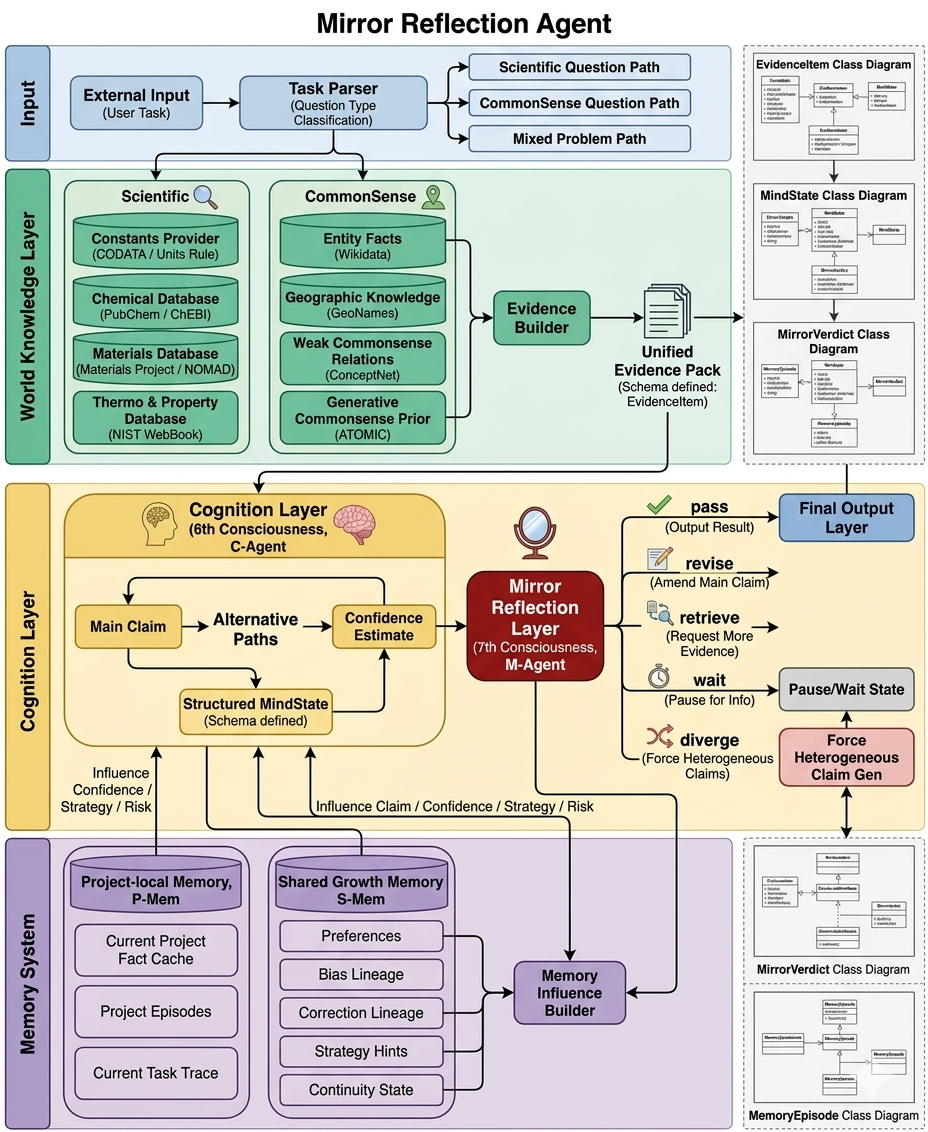
\includegraphics[width=\textwidth]{figure1_architecture.png}
\caption{Overall engineering schematic of Mirror Reflection Agent. The figure shows the relation between the scientific knowledge layer, commonsense knowledge layer, cognition layer, mirror reflection layer, and memory system.}
\label{fig:architecture}
\end{figure}

\subsection{Scientific Knowledge Layer}

The scientific layer is responsible for higher-confidence, condition-sensitive evidence. Its role is to parse scientific entity/property questions, resolve entities and normalize units, route across structured scientific sources, and build evidence packs with provenance and warnings. This layer is the source of hard constraints.

\subsection{Commonsense Knowledge Layer}

The commonsense layer is responsible for softer background priors. Its role is to resolve general entities and relations, provide context when prompts rely on implicit world knowledge, and distinguish structured facts from weak commonsense priors. This layer should not be treated as equivalent to scientific evidence. Its proper role is contextual support, not unrestricted claim justification.

\subsection{Cognition Layer}

The cognition layer builds a structured \texttt{MindState} containing current input, task goal, main claim, evidence, hidden assumptions, alternative paths, confidence, self-risk, proposed action, and self-state. This step externalizes an otherwise opaque intermediate draft.

\subsection{Mirror Layer}

The mirror layer reviews the \texttt{MindState} and returns a \texttt{MirrorVerdict}. Current implemented checks include premature convergence, concept blending, evidence gap, overclaiming, weak commonsense presented as fact, structured-fact priority violation, unit inconsistency, condition-scope violations, stale template reuse, and divergence need. The mirror is best understood as a reliability governor rather than a semantic truth oracle.

\subsection{Memory Layer}

The memory layer contains project-local memory and optional shared-growth memory. The key memory signals are fact hints, context hints, bias alerts, correction hints, strategy hints, and divergence triggers. This gives the architecture a notion of bounded continuity across runs while keeping memory inspectable and auditable.

\subsection{Implemented Versus Planned Scope}

One source of potential confusion in the current manuscript is the difference between the full architecture sketch and the subset that is exercised by the current pilot benchmark. Table~\ref{tab:implemented-scope} makes that distinction explicit. The current paper evaluates the implemented orchestration loop, mirror logic, local memory, optional dual-layer shared memory, and replayable audit path. The broader scientific-source ecosystem shown in the architecture figure should be interpreted as the intended system envelope rather than as a claim that every source or route is already validated in the present experiments.

\begin{table}[H]
\centering
\begin{tabular}{p{4.0cm}p{2.2cm}p{2.2cm}p{5.0cm}}
\toprule
Component & Status & Exercised in pilot & Current role \\
\midrule
Structured \texttt{MindState} generation & implemented & yes & candidate cognition state before final output \\
Typed mirror verdicts & implemented & yes & revise/retrieve/wait/diverge/pass control \\
Project-local memory & implemented & yes & correction and strategy retrieval \\
Shared-growth memory & implemented & yes & advisory cross-run correction support in dual-layer mode \\
Replayable audit trace & implemented & yes & reproducibility and case inspection \\
Scientific source routing ecosystem & partial / planned & not fully & intended evidence expansion for future science-facing benchmark \\
Large multi-source scientific QA workflow & planned & no & next-stage benchmark target rather than current validated scope \\
\bottomrule
\end{tabular}
\caption{Implemented versus planned scope of the architecture. This table separates the validated control loop from the larger system envelope suggested by the architecture figure.}
\label{tab:implemented-scope}
\end{table}

\section{Methods}

The current implementation is deterministic in its control structure. A run begins by building memory influence from prior episodes, then constructing scientific and commonsense evidence packs, then generating a candidate \texttt{MindState}. The mirror layer reviews that state and emits one of five verdicts: \texttt{pass}, \texttt{revise}, \texttt{retrieve}, \texttt{wait}, or \texttt{diverge}. If the verdict is \texttt{pass}, the system returns a bounded output and writes a memory episode. If the verdict is \texttt{revise}, the cognition layer rewrites the claim under mirror guidance. If the verdict is \texttt{retrieve}, memory signals are refreshed and re-applied. If the verdict is \texttt{diverge}, the system is forced to adopt a different explanatory scaffold. If the verdict is \texttt{wait}, the system emits a deferred answer.

This structure matters for evaluation because it allows multiple reliability phenomena that are usually conflated in end-to-end generations to be separated analytically: evidence insufficiency, stale-template reuse, prior-correction reuse, condition-scope violations, and calibrated abstention.

\section{Experimental Setting}

The present paper reports a pilot evaluation using the existing repository benchmark and then outlines a feasible expansion path for a solo researcher. The experimental objective is not to show that the architecture outperforms frontier foundation models on raw scientific capability. The objective is to show that, holding the underlying model and implementation family fixed, explicit critique control and correction-lineage memory improve reliability-oriented behavior. The manuscript therefore treats the current experiments as proof-of-mechanism evidence and not as a definitive scientific benchmark.

\subsection{Experimental Questions}

The current manuscript is organized around three concrete questions. First, does dual-layer memory reduce premature convergence relative to local-only memory? Second, does structured correction lineage improve retention of prior corrections under reworded prompts? Third, does the added memory layer preserve already-good bounded behavior without introducing shared-memory pollution? These questions are narrow enough to be answered by the present implementation and directly reflect the architecture's intended purpose.

\subsection{Pilot Hypotheses}

The pilot benchmark tests the following hypotheses.

\begin{itemize}[leftmargin=1.2em]
\item \textbf{H1:} dual-layer memory lowers premature convergence.
\item \textbf{H2:} dual-layer memory improves correction retention.
\item \textbf{H3:} dual-layer memory improves revision success without increasing shared-memory pollution.
\item \textbf{H4:} bounded-control cases remain stable rather than degrading under the richer memory setting.
\end{itemize}

\subsection{Pilot Benchmark}

We ran the existing repository benchmark directly without modifying the evaluation harness:

\begin{center}
\texttt{python3 -m evals.run\_evals --format json}
\end{center}

The current benchmark contains four cases and compares a \texttt{local\_only} configuration against a \texttt{dual\_layer} configuration. The cases target concept blending, premature convergence, project-local precedence, and bounded control behavior.

All pilot metrics are computed by deterministic rules in the repository evaluation harness rather than by an external LLM judge. This design keeps the present benchmark transparent and replayable, although it also means that metric coverage is narrower than what will be needed in a larger benchmark study.

\subsection{Expanded Evaluation Plan}

For a larger study, the most informative comparison is architecture-first rather than model-first. The recommended ablations are direct answer, structured cognition only, mirror without memory, mirror with local memory, and mirror with dual-layer memory. A practical benchmark can combine three tracks:

\begin{itemize}[leftmargin=1.2em]
\item an internal reliability set covering concept blending, premature convergence, correction retention, and memory pollution
\item a small scientific QA set with 100--300 manually curated condition-sensitive questions
\item a longitudinal correction set that repeats related prompt families across sessions
\end{itemize}

The expanded evaluation is feasible with local 7B--14B instruction-tuned models, rented single-GPU cloud instances for batch runs, and API baselines only for a limited comparison slice.

\begin{table}[H]
\centering
\begin{tabular}{p{2.2cm}p{3.6cm}p{3.5cm}p{3.6cm}}
\toprule
Track & Task family & Planned baselines & Primary metrics \\
\midrule
Track A & internal reliability benchmark & direct answer, cognition only, mirror only, local memory, dual-layer memory & revision success, correction retention, premature convergence, pollution risk \\
Track B & condition-sensitive scientific QA & same architecture-first ablations & correctness, condition preservation, unit consistency, abstention quality \\
Track C & longitudinal correction benchmark & local memory versus dual-layer memory & cross-session correction retention, error recurrence reduction, conflict handling \\
\bottomrule
\end{tabular}
\caption{Planned next-round benchmark protocol. The table defines the minimum evidence needed to move beyond the current pilot proof-of-mechanism.}
\label{tab:planned-benchmark}
\end{table}

\section{Results}

\subsection{Metric Summary}

\begin{table}[H]
\centering
\begin{tabular}{lccc}
\toprule
Metric & local\_only & dual\_layer & delta \\
\midrule
Premature convergence rate & 1.000 & 0.000 & -1.000 \\
Revision success rate & 0.500 & 1.000 & +0.500 \\
Correction retention rate & 0.000 & 1.000 & +1.000 \\
Shared-memory pollution risk & 0.000 & 0.000 & 0.000 \\
Average confidence & 0.6075 & 0.5625 & -0.0450 \\
\bottomrule
\end{tabular}
\caption{Pilot benchmark summary from the existing implementation.}
\label{tab:current-results}
\end{table}

\begin{figure}[H]
\centering
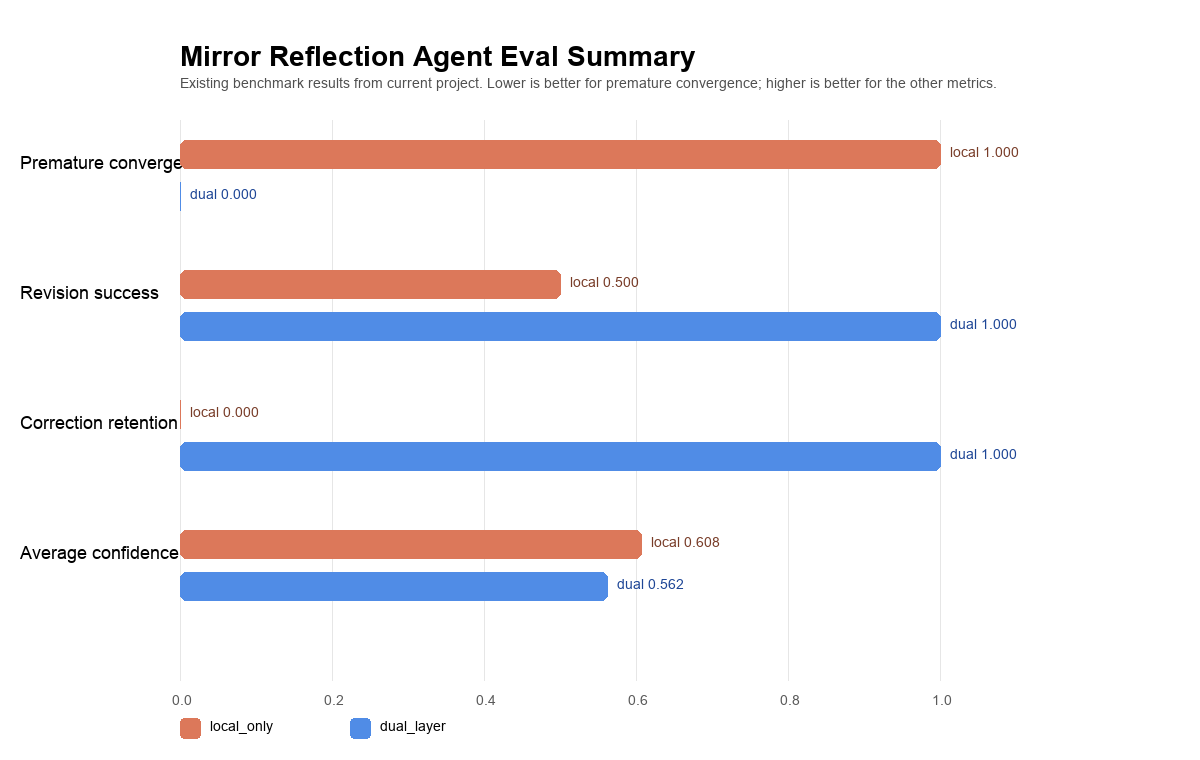
\includegraphics[width=\textwidth]{figure2_results.png}
\caption{Summary plot of the current benchmark. The dual-layer setting eliminates premature convergence in the current suite and substantially improves revision success and correction retention, while slightly reducing average confidence.}
\label{fig:benchmark}
\end{figure}

\subsection{Analysis of the Pilot Figure}

Figure~\ref{fig:benchmark} captures the current logic of the paper clearly. The main gain is not that dual-layer memory makes the system more assertive. It makes the system more controlled. Premature convergence drops from 1.000 to 0.000, which means the architecture is less likely to lock into an overconfident conclusion too early. Revision success rises from 0.500 to 1.000, indicating that the mirror-plus-memory loop is not only triggering revisions but helping those revisions land in a safer final state. Correction retention rises from 0.000 to 1.000, which supports the central claim that structured correction lineage can influence later behavior in a measurable way. Average confidence decreases slightly from 0.6075 to 0.5625; in this setting that should be interpreted as improved calibration rather than degradation, because the target behavior is bounded reliability rather than maximal certainty.

\subsection{Case-Level Interpretation}

In \texttt{concept\_blending\_shared\_recovery}, dual-layer memory retained the target correction while local-only did not. In \texttt{premature\_convergence\_shared\_bias\_alert}, dual-layer memory removed premature convergence and preserved the shared correction signal. In \texttt{project\_local\_precedence}, the system preserved project-local strategy priority while still using shared memory as advisory context. In \texttt{bounded\_control\_case}, dual-layer memory did not degrade already-good behavior.

\begin{table}[H]
\centering
\begin{tabular}{lcccc}
\toprule
Case & Mode & Verdict & Revisions & Correction retained \\
\midrule
Concept blending recovery & local\_only & pass & 1 & no \\
Concept blending recovery & dual\_layer & pass & 2 & yes \\
Premature convergence alert & local\_only & wait & 4 & no \\
Premature convergence alert & dual\_layer & wait & 4 & yes \\
Project-local precedence & local\_only & pass & 0 & yes \\
Project-local precedence & dual\_layer & pass & 0 & yes \\
Bounded control case & local\_only & pass & 0 & yes \\
Bounded control case & dual\_layer & pass & 0 & yes \\
\bottomrule
\end{tabular}
\caption{Case-level outcomes in the pilot benchmark.}
\label{tab:case-breakdown}
\end{table}

\begin{figure}[H]
\centering
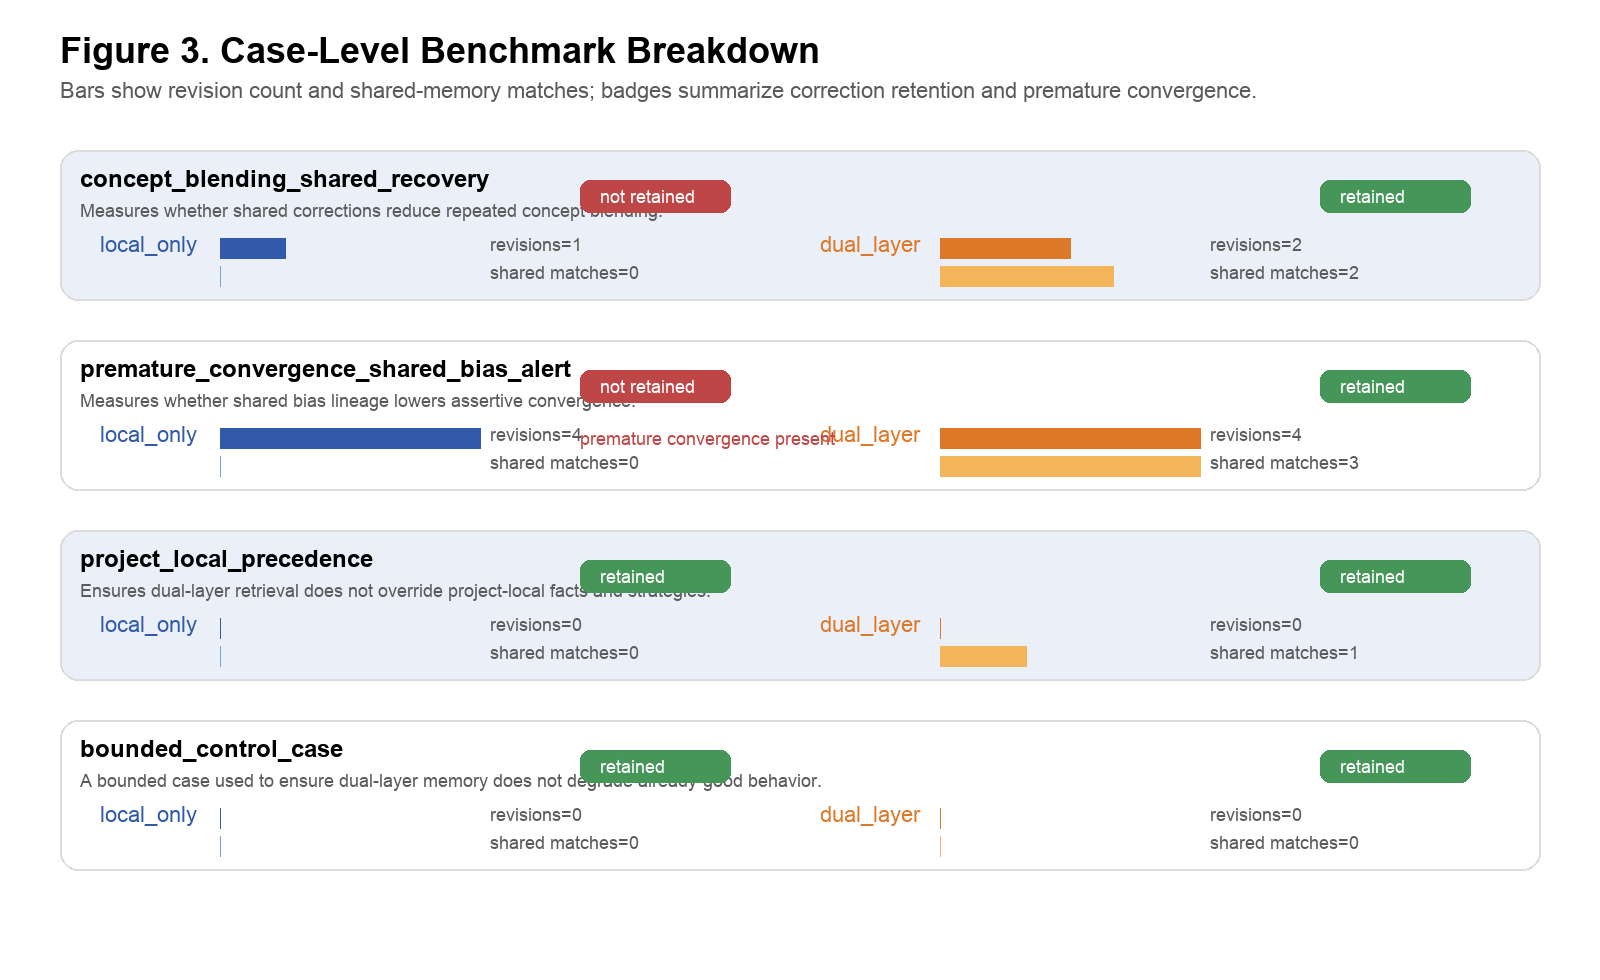
\includegraphics[width=\textwidth]{figure3_case_breakdown.png}
\caption{Case-level mechanism breakdown. Bars summarize revision counts and shared-memory matches, while badges indicate whether the target correction was retained.}
\label{fig:case-breakdown}
\end{figure}

\subsection{Analysis of Case-Level Mechanisms}

Figure~\ref{fig:case-breakdown} and Table~\ref{tab:case-breakdown} make the mechanism-level story more explicit. The strongest effect appears in the two error-recovery cases. In the concept-blending case, dual-layer memory performs one additional revision and retrieves two shared matches, which is sufficient to retain the target correction while avoiding a stronger consciousness claim. In the premature-convergence case, both modes reach a \texttt{wait} verdict after four revisions, but only dual-layer memory retains the explicit shared correction and clears the premature-convergence flag. The remaining two cases show the boundary conditions of the architecture: project-local precedence is preserved, and already-bounded behavior is not degraded by the richer memory mode.

\subsection{Repeated-Run Stability}

To check whether the pilot pattern is merely a one-off artifact, we repeated the benchmark for five iterations using the repository's built-in averaging mode:

\begin{center}
\texttt{python3 -m evals.run\_evals --iterations 5 --format json}
\end{center}

Across five iterations, the reported aggregate metrics remained unchanged. In the current implementation this indicates deterministic behavior under the pilot benchmark and supports the reproducibility of the current tables and figures. The repeated-run stability result is modest, but it matters for this paper because a reliability-control architecture should not depend on accidental metric drift across identical runs.

\subsection{Interpretation of the Current Evidence}

The present results do not establish broad scientific superiority. They support a narrower and more credible claim: the architecture improves reliability-oriented behavior under correction and memory. That is the appropriate level of claim for the current stage of the project.

\section{Discussion}

The current benchmark is intentionally small, but it already reveals the kind of gain that matters for this architecture. The system becomes less prone to premature commitment, more likely to preserve prior corrections, and more willing to trade raw confidence for bounded behavior. For a scientific assistant, that trade is desirable. A slightly less confident answer that respects evidence limits is often more valuable than a fluent but overgeneralized one. At the same time, the pilot should be read as evidence about control logic, not as evidence that the full scientific-knowledge envelope in Figure~\ref{fig:architecture} has already been validated.

The results also suggest that the architecture is especially well suited to settings where the central risk is not random error, but recurrent patterned error. In those cases, correction-lineage memory and verdict-typed control give the system a mechanism for avoiding the same mistake under a new wording. That is a more realistic notion of practical improvement than simply raising one-shot answer accuracy on a static benchmark.

\subsection{What the Current Pilot Already Shows}

Even with only four benchmark cases, the present evidence is best interpreted as a proof-of-mechanism result rather than a broad benchmark victory. The manuscript does not need to argue that the architecture solves scientific reasoning in general. It needs to establish that the architecture alters reliability behavior in the intended direction. On that criterion, the current pilot is encouraging: dual-layer memory removes premature convergence in the targeted case, improves revision success, retains shared corrections in the intended settings, and does not increase shared-memory pollution.

\subsection{Next Experimental Round}

The next round of experiments should expand breadth rather than change the paper's claim. The clearest path is to add a small condition-sensitive scientific QA benchmark, then pair it with the same ablation logic used here. That would allow the manuscript to move from proof-of-mechanism to a stronger AI-for-Science reliability demonstration without changing the architecture's central contribution.

\subsection{Blind Spots}

The present system still has important limits. The agent can reuse corrections, but it does not autonomously redesign its own rules, objectives, or schema. That is controlled adaptation, not full self-improvement. The memory system preserves structured lessons, but it does not yet maintain rich multi-session dialogue continuity with evolving user preferences, conceptual drift, and conflict resolution. The mirror works well on explicit risks such as overclaiming or evidence gaps, but may still miss subtle errors in decomposition, framing, or hidden variable choice.

\subsection{Why Local Models Matter}

The broader deployment trend toward local models strengthens the case for this architecture. In many scientific or institutional settings, data governance, privacy, latency, and cost place practical limits on heavy cloud-only workflows. A reliability-control architecture that can wrap modest local models is therefore attractive because it shifts some performance gains from model scale to system design. In that setting, the question is not only how strong the base model is, but how well the overall system knows when to revise, abstain, retrieve, and reuse prior corrections.

\section{Limitations}

The current prototype does not yet demonstrate strong continual learning, robust multi-session conversational identity, broad scientific discovery ability, or comprehensive critique coverage for all failure modes. The pilot benchmark is small and should be treated as proof-of-mechanism rather than as a broad benchmark victory. The architecture also depends on the quality of its critique rules and memory writes; poor mirror coverage or noisy lessons could reduce reliability rather than improve it. In addition, the present manuscript does not yet include the full ablation chain proposed in Table~\ref{tab:planned-benchmark}, nor does it yet validate condition-sensitive scientific QA at a scale sufficient for a strong AI-for-Science claim.

\section{Conclusion}

Mirror Reflection Agent is best understood as a structured reliability-control architecture rather than a claim about machine consciousness or autonomous scientific discovery. Its value lies in externalizing intermediate cognition, enforcing typed critique decisions, and preserving correction lineage across runs. The current implementation supports a bounded pilot narrative: less premature convergence, stronger revision success, and better correction retention under bounded confidence. The paper's strongest present contribution is therefore architectural and methodological: it defines an inspectable control loop and shows, on a small replayable benchmark, that this loop changes reliability behavior in the intended direction. The next stage of the work is to validate the same control logic on a condition-sensitive scientific benchmark with fuller ablations and richer artifact release.

\section*{Data and Code Availability}

The implementation, pilot evaluation harness, manuscript sources, and generated figures are maintained in the local project repository used for this study. The current pilot metrics reported in this manuscript are reproduced from the repository evaluation commands described in Section 5. The generated benchmark assets include a single-run raw dump, a five-iteration repeated-run dump, a text case breakdown, and the corresponding manuscript figures.

\begin{thebibliography}{9}
\bibitem{selfrefine}
Madaan A, Tandon N, Clark P et al. 2023 Self-Refine: Iterative Refinement with Self-Feedback. arXiv:2303.17651.

\bibitem{reflexion}
Shinn N, Cassano F, Berman E and Labash B 2023 Reflexion: Language Agents with Verbal Reinforcement Learning. arXiv:2303.11366.

\bibitem{critic}
Gou Z, Shao Z, Gong Y et al. 2024 CRITIC: Large Language Models Can Self-Correct with Tool-Interactive Critiquing. arXiv:2305.11738.

\bibitem{selfrag}
Asai A, Wu Z, Wang Y et al. 2024 Self-RAG: Learning to Retrieve, Generate, and Critique through Self-Reflection. arXiv:2310.11511.

\bibitem{sofai}
Bergamaschi Ganapini M, Campbell M, Fabiano F et al. 2025 Fast, slow, and metacognitive thinking in AI. npj Artificial Intelligence 1, 27.

\bibitem{academicresponse}
Sun Z, Zhang Y, Liu X et al. 2025 Self-reflection enhances large language models towards substantial academic response. npj Artificial Intelligence 1, 45.
\end{thebibliography}

\end{document}
